\chapter{测试与分析}\label{chap:result}

硬件设计完成之后,首先需要经过综合,综合阶段主要查看资源利用率情况确保资源足够。此外,Vivado 还会构建出理想的时钟树,给出理想的 Timing 和功耗报告。但综合阶段的数字电路设计没有映射到实际的物理器件上,所以这部分将基于实现阶段的 Timing 与功耗进行分析。

\section{资源利用率}

在硬件设计实现章节,本设计将 NVDLA 内部数量庞大的存储资源替换为了 FPGA 片上的 BRAM 资源,在替换之前,其资源利用率情况如表~\ref{tab:Resource Report Before}所示。

\begin{table}[!htbp]
    \caption{优化 RAM 之前的资源利用率}
    \label{tab:Resource Report Before}
    \centering
    \footnotesize% fontsize
    \setlength{\tabcolsep}{4pt}% column separation
    \renewcommand{\arraystretch}{1.2}%row space 
    \begin{tabular}{llll}
        \toprule
        \textbf{RESOURCE} & \textbf{UTILIZATION} & \textbf{AVAILABLE} & \textbf{Utilization \%} \\
        \midrule
        LUT               & 421698               & 218600               & 192.91                  \\
        LUTRAM            & 8                    & 70400                & 0.01                    \\
        FF                & 92622                & 437200               & 22.33                   \\
        DSP               & 33                   & 900                  & 3.67                    \\
        BUFG              & 12                   & 32                   & 37.5                    \\
        \bottomrule                   
    \end{tabular}
\end{table}

此时发现,LUT 资源的使用严重超过可使用数量,而 FPGA 内部的 BRAM 资源几乎未被使用,经过优化后,本设计的资源利用率信息最终如表~\ref{tab:Resource Report},资源的使用情况都在合理范围之内。

\begin{table}[!htbp]
    \caption{资源利用率}
    \label{tab:Resource Report}
    \centering
    \footnotesize% fontsize
    \setlength{\tabcolsep}{4pt}% column separation
    \renewcommand{\arraystretch}{1.2}%row space 
    \begin{tabular}{llll}
        \toprule
        \textbf{RESOURCE} & \textbf{UTILIZATION} & \textbf{AVAILABLE} & \textbf{Utilization \%} \\
        \midrule
        LUT               & 80293                & 218600               & 36.73                   \\
        LUTRAM            & 1015                 & 70400                & 1.44                    \\
        FF                & 92678                & 437200               & 21.20                   \\
        BRAM              & 95                   & 545                  & 17.43                   \\
        DSP               & 42                   & 900                  & 4.67                    \\
        BUFG              & 1                    & 32                   & 3.13                    \\
        \bottomrule                   
    \end{tabular}
\end{table}

\section{最大工作频率分析}

静态时序分析(Static Timing Analysis,STA)的基本功能是对设计电路的时序进行检查。如图~\ref{fig:Setup and Hold}所示,时序检查是指建立时间与保持时间检查:

\begin{itemize}
    \item 建立时间即$t_{setup}$,检查该时间是为了保证数据可以在给定时钟周期内到达触发器,如果建立时间无法满足,则触发器会在数据到达之前采集到错误的数据。
    \item 保持时间即$t_{hold}$,检查该时间是为了保证数据在被触发器采样后还能保持一定时间,如果保持时间无法满足,则触发器会采集到滞后的数据。
\end{itemize}

\begin{figure}[!htbp]
    \centering
    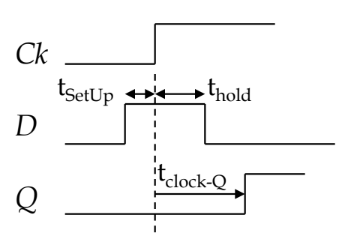
\includegraphics[width=0.4\textwidth]{SetupAndHold.png}
    \caption{Setup 和 Hold 示例}
    \label{fig:Setup and Hold}
\end{figure}

一个数字电路中只要存在环路边界,就会存在理论上的最大工作频率。时序检查的目的都是为了保证触发器可以发送并且采样到正确的数据,确保电路输入的时钟频率在理论的最大频率之下。

首先将 10Mhz 的时钟接入 NVDLA,实现之后的 Timing 报告如表~\ref{tab:10Mhz Timing}所示,其中 Slack 指的是建立时间与到达时间的差值,如果整个设计的 Slack 存在负值,则就存在部分寄存器无法获取到数据,电路无法正常工作。从该表中可以看出,对于 Setup Slack,设计的关键路径保有 88.126 ns 的余量,而关键路径的 Hold Slack 只有 0.030 ns 的余量,不存在负数,电路可以正常工作。

\begin{table}[!htbp]
    \caption{10 Mhz 情况下的关键路径时序情况}
    \label{tab:10Mhz Timing}
    \centering
    \footnotesize% fontsize
    \setlength{\tabcolsep}{4pt}% column separation
    \renewcommand{\arraystretch}{1.2}%row space 
    \begin{tabular}{llll}
        \toprule
        \textbf{Frequency}        & \textbf{Worst Setup Slack}    & \textbf{Worst Hold Slack}    & \textbf{Total Negative Slack} \\
        \midrule
        \multicolumn{1}{c}{10Mhz} & \multicolumn{1}{c}{88.126 ns} & \multicolumn{1}{c}{0.030 ns} & \multicolumn{1}{c}{0.000 ns} \\
        \bottomrule                   
    \end{tabular}
\end{table}

本设计在分析 NVDLA 最大工作时钟时,选取了几个典型的时钟值,分别是 25Mhz、50Mhz、75Mhz、100Mhz,他们的关键路径的时钟情况如表~\ref{tab:25-100 Mhz Timing}所示,可以发现当时钟频率不断增加的时候,关键路径的 Slack 值不断在变小,影响 NVDLA 工作的主要问题是 Setup 时间不足,在 100Mhz 的时候已经不足 1 ns。

\begin{table}[!htbp]
    \caption{不同时钟下的关键路径时序情况}
    \label{tab:25-100 Mhz Timing}
    \centering
    \footnotesize% fontsize
    \setlength{\tabcolsep}{4pt}% column separation
    \renewcommand{\arraystretch}{1.2}%row space 
    \begin{tabular}{cccc}
        \toprule
        \multicolumn{1}{l}{\textbf{Frequency}} & \multicolumn{1}{l}{\textbf{Worst Setup Slack}} & \multicolumn{1}{l}{\textbf{Worst Hold Slack}} & \multicolumn{1}{l}{\textbf{Total Negative Slack}} \\
        \midrule
        25Mhz                                  & 29.048 ns                                      & 0.021 ns                                      & 0.000 ns                                          \\
        50Mhz                                  & 9.959 ns                                       & 0.007 ns                                      & 0.000 ns                                          \\
        75Mhz                                  & 3.832 ns                                       & 0.028 ns                                      & 0.000 ns                                          \\
        100Mhz                                 & 0.751 ns                                       & 0.030 ns                                      & 0.000 ns                                          \\
        \bottomrule                   
    \end{tabular}
\end{table}

如表~\ref{tab:150 Mhz Timing}所示,将时钟再提升至 150Mhz,则时钟已经出现了违例,具体表现为最差路径的 Slack 为负值,电路无法正常工作。此时强行上板会导致时序混乱,造成读写相关的寄存器失败。

由以上分析,在本设计中给 NVDLA 的输入时钟为 100Mhz,但是在 FPGA 上工作的最大时钟不代表进行 ASIC 设计能够工作的最大时钟,例如 Jetson Xavier NX 板卡上的 NVDLA 的工作时钟为 600 Mhz,根据中国科学院信息工程研究所的流片经验,其工作时钟为 800Mhz。

\begin{table}[!htbp]
    \caption{150 Mhz 情况下的关键路径时序情况}
    \label{tab:150 Mhz Timing}
    \centering
    \footnotesize% fontsize
    \setlength{\tabcolsep}{4pt}% column separation
    \renewcommand{\arraystretch}{1.2}%row space 
    \begin{tabular}{llll}
        \toprule
        \textbf{Frequency}         & \textbf{Worst Setup Slack}    & \textbf{Worst Hold Slack}    & \textbf{Total Negative Slack} \\
        \midrule
        \multicolumn{1}{c}{150Mhz} & \multicolumn{1}{c}{-0.324 ns} & \multicolumn{1}{c}{0.033 ns} & \multicolumn{1}{c}{-9.728 ns} \\
        \bottomrule                   
    \end{tabular}
\end{table}

如表~\ref{tab:10-100 Mhz Power},本文还给出了 10Mhz、25Mhz、50Mhz、75Mhz、100Mhz 时钟下的功耗情况,当时钟频率增加的时候,系统的功耗不断增加,其中静态功耗占比较小,约为 10\%,动态功耗的占比较大,约为 90\%。

\begin{table}[!htbp]
    \caption{10 25 50 75 100 Mhz 功耗}
    \label{tab:10-100 Mhz Power}
    \centering
    \footnotesize% fontsize
    \setlength{\tabcolsep}{4pt}% column separation
    \renewcommand{\arraystretch}{1.2}%row space 
    \begin{tabular}{cccc}
        \toprule
        \multicolumn{1}{l}{\textbf{Frequency}} & \multicolumn{1}{l}{\textbf{Total Power}} & \multicolumn{1}{l}{\textbf{Static Power}} & \multicolumn{1}{l}{\textbf{Dynamic Power}} \\
        \midrule
        10Mhz                                  & 1.805W                                   & 0.220W(12.2\%)                            & 1.585W(87.8\%)                             \\
        25 Mhz                                 & 1.921W                                   & 0.221W(11.5\%)                            & 1.700W(88.5\%)                             \\
        50 Mhz                                 & 2.129W                                   & 0.223W(10.5\%)                            & 1.906W(89.5\%)                             \\
        75 Mhz                                 & 2.325W                                   & 0.224W(9.6\%)                             & 2.101W(90.4\%)                             \\
        100 Mhz                                & 2.528W                                   & 0.226W(8.9\%)                             & 2.302W(91.9\%)                             \\
        \bottomrule                   
    \end{tabular}
\end{table}

\section{基于 NVDLA 的硬件加速系统性能评估}

\subsection{实验配置}

前文中提到,本设计基于 Caffe 框架自行训练了三个网络,其网络结构限于篇幅,全部的 prototxt 文件与 loadables 文件详见 Github\cite{nvdla_loadables}。此外,为了对比 CPU 的运行时间,本设计还在 ARM A9 处理器上进行了 Caffe 框架的移植与编译,对预训练的 Caffemodel 进行 CPU 侧的推理,由于 CPU 的访存特性,Caffe 在进行推理的时候速度会由慢到快,最终趋于稳定,所以本设计取迭代五十次后取推理时间的平均值。如图~\ref{fig:BootStrap}所示,本节还在主机端基于 Bootstrap 与 JQuery 等 Web 应用技术开发了的网页服务,并通过 Ajax 向后端发送推理请求,运行在 ZYNQ 7000+ 芯片上的 Ubuntu 操作系统里,使用 Flask 框架接受请求并且调度。但是在实际测试过程中,如进行数据集级别的推理以及与 Caffe 进行比较,均不在该网页服务里完成。

\begin{figure}[!htbp]
    \centering
    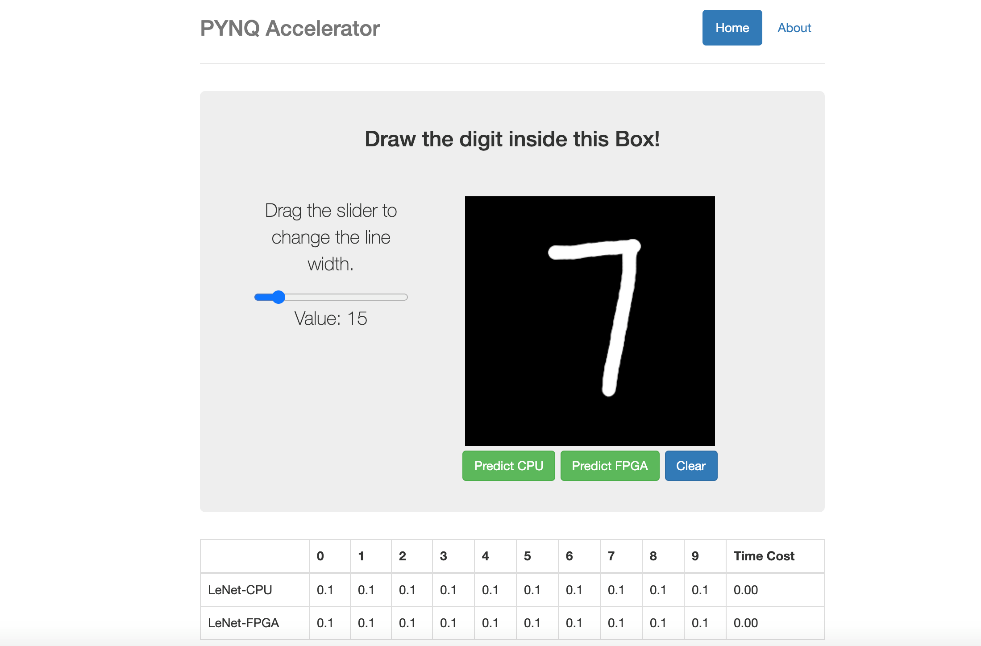
\includegraphics[width=0.7\textwidth]{bootstrap}
    \caption{用户友好的输入页面}
    \label{fig:BootStrap}
\end{figure}

\subsection{精度对比分析}

本节将 TensorRT 为了量化而采样的一千张图像再次使用 NVDLA 进行推理并验证精度是否存在损失。其中,Resnet18-IMAGENET2012 网络参数较多,而本设计仅有 500MB 左右的片上存储,使得该网络无法在开发板卡上正常推理,精度的得出是使用的 QEMU 虚拟环境,经过 HPC 模拟硬件加速器调度得出。

\begin{table}[!htbp]
    \caption{精度对比}
    \label{tab:Qualifications Report}
    \centering
    \footnotesize% fontsize
    \setlength{\tabcolsep}{4pt}% column separation
    \renewcommand{\arraystretch}{1.2}%row space 
    \begin{tabular}{lccc}
        \toprule
        \textbf{Network}      & \multicolumn{1}{l}{\textbf{Valiadation Accuracy \%}} & \multicolumn{1}{l}{\textbf{Calibration Accuracy \%}}  & \multicolumn{1}{l}{\textbf{NVDLA Accuracy \%}} \\
        \midrule
        Lenet5-MNIST          & 99.7                                                 & 99.5                                                 & 97.5                                                 \\  
        Resnet18-CIFAR10      & 90.2                                                 & 86.7                                                 & 80.7                                                 \\
        Resnet18-IMAGENET2012 & 60.2(Top5)                                           & 50.5(Top5)                                           & 50.5(Top5)                                           \\
        \bottomrule                   
    \end{tabular}
\end{table}

\textbf{实验结论:}理论上,NVDLA 的精度应该与 TensorRT 量化之后的精度一致,但是实际测试中,NVDLA的量化精度稍微低一些。经过分析,是因为 Caffe 训练的模型内部使用 OpenCV 进行图像读取操作,而 OpenCV 读取的图像为 BGR 格式,在 NVDLA 的 Runtime 阶段,由于 BGR 转 RGB 的操作会引发一系列错误,所以本设计将该操作去除,影响了部分精度,而 Resnet18-IMAGENET2012 未进行该处理,精度保持一致。

\subsection{推理速度分析}

本节针对设计的三个模型统计 NVDLA 的推理速度,其中Resnet18-IMAGENET2012 因为需要分配的内存过大,而无法在板卡上运行,所以本设计没有对运行速度进行评估,其余两个模型,分别推理了一千张图像观察推理的平均耗时。


\begin{table}[!htbp]
    \caption{运行速度}
    \label{tab:Execution Time}
    \centering
    \footnotesize% fontsize
    \setlength{\tabcolsep}{4pt}% column separation
    \renewcommand{\arraystretch}{1.2}%row space 
    \begin{tabular}{lcccc}
        \toprule
        \textbf{Network}                                   & \multicolumn{1}{l}{\textbf{1000 Images Execution Time}} & \multicolumn{1}{l}{\textbf{Time Per Image}} & \textbf{FPS}     & \multicolumn{1}{l}{\textbf{Time ARM A9 (666 Mhz)}} \\
        \midrule
        \textbf{Lenet5-MNIST}          & 288129 ms                                               & 288.13 ms                                   & 3.47             & 23.55 ms                                            \\
        \textbf{Resnet18-CIFAR10}      & 287145 ms                                               & 287.15 ms                                   & 3.48             & 342.24 ms                                          \\
        \textbf{Resnet18-IMAGENET2012} & \textbackslash{}                                        & \textbackslash{}                            & \textbackslash{} & 6169.63 ms                                         \\
        \bottomrule                   
    \end{tabular}
\end{table}

\textbf{实验结论:}如表~\ref{tab:Execution Time}所示,
虽然根据图表所示,对于 Lenet5,CPU 侧的推理仅需要 20ms,其速度比设计的硬件加速器还要快 10 倍,究其原因如下:

\begin{enumerate}
    \item CPU 是集成在 ZYNQ 器件上的硬核处理器,主频可达到 666 Mhz、而 NVDLA 因为其在 FPGA 上运行导致最高运行频率收到限制,仅可达到 100 Mhz。
    \item 对于 NVDLA,因其在 FPGA 上实现,所以功能验证正确是最主要的,对于运行速度需要通过 ASIC 流程得出,根据中国科学院自动化研究所的研究,在 600 Mhz 的工作频率下,Lenet5 的推理速度可以达到 0.2 ms \cite{9040769}。 
\end{enumerate}

其次,Resnet18-CIFAR10 在 CPU 侧推理的速度是 Lenet5 的 14.5 倍,可知其网络比 Lenet5 复杂许多,但是在 NVDLA 侧,推理速度仍然与 Lenet5 不相上下,说明在这两个网络的推理过程中,网络的复杂程度不是影响推理速度的关键因素,可能是访存等其他原因。